\documentclass[1p]{elsarticle_modified}
%\bibliographystyle{elsarticle-num}

%\usepackage[colorlinks]{hyperref}
%\usepackage{abbrmath_seonhwa} %\Abb, \Ascr, \Acal ,\Abf, \Afrak
\usepackage{amsfonts}
\usepackage{amssymb}
\usepackage{amsmath}
\usepackage{amsthm}
\usepackage{scalefnt}
\usepackage{amsbsy}
\usepackage{kotex}
\usepackage{caption}
\usepackage{subfig}
\usepackage{color}
\usepackage{graphicx}
\usepackage{xcolor} %% white, black, red, green, blue, cyan, magenta, yellow
\usepackage{float}
\usepackage{setspace}
\usepackage{hyperref}

\usepackage{tikz}
\usetikzlibrary{arrows}

\usepackage{multirow}
\usepackage{array} % fixed length table
\usepackage{hhline}

%%%%%%%%%%%%%%%%%%%%%
\makeatletter
\renewcommand*\env@matrix[1][\arraystretch]{%
	\edef\arraystretch{#1}%
	\hskip -\arraycolsep
	\let\@ifnextchar\new@ifnextchar
	\array{*\c@MaxMatrixCols c}}
\makeatother %https://tex.stackexchange.com/questions/14071/how-can-i-increase-the-line-spacing-in-a-matrix
%%%%%%%%%%%%%%%

\usepackage[normalem]{ulem}

\newcommand{\msout}[1]{\ifmmode\text{\sout{\ensuremath{#1}}}\else\sout{#1}\fi}
%SOURCE: \msout is \stkout macro in https://tex.stackexchange.com/questions/20609/strikeout-in-math-mode

\newcommand{\cancel}[1]{
	\ifmmode
	{\color{red}\msout{#1}}
	\else
	{\color{red}\sout{#1}}
	\fi
}

\newcommand{\add}[1]{
	{\color{blue}\uwave{#1}}
}

\newcommand{\replace}[2]{
	\ifmmode
	{\color{red}\msout{#1}}{\color{blue}\uwave{#2}}
	\else
	{\color{red}\sout{#1}}{\color{blue}\uwave{#2}}
	\fi
}

\newcommand{\Sol}{\mathcal{S}} %segment
\newcommand{\D}{D} %diagram
\newcommand{\A}{\mathcal{A}} %arc


%%%%%%%%%%%%%%%%%%%%%%%%%%%%%5 test

\def\sl{\operatorname{\textup{SL}}(2,\Cbb)}
\def\psl{\operatorname{\textup{PSL}}(2,\Cbb)}
\def\quan{\mkern 1mu \triangleright \mkern 1mu}

\theoremstyle{definition}
\newtheorem{thm}{Theorem}[section]
\newtheorem{prop}[thm]{Proposition}
\newtheorem{lem}[thm]{Lemma}
\newtheorem{ques}[thm]{Question}
\newtheorem{cor}[thm]{Corollary}
\newtheorem{defn}[thm]{Definition}
\newtheorem{exam}[thm]{Example}
\newtheorem{rmk}[thm]{Remark}
\newtheorem{alg}[thm]{Algorithm}

\newcommand{\I}{\sqrt{-1}}
\begin{document}

%\begin{frontmatter}
%
%\title{Boundary parabolic representations of knots up to 8 crossings}
%
%%% Group authors per affiliation:
%\author{Yunhi Cho} 
%\address{Department of Mathematics, University of Seoul, Seoul, Korea}
%\ead{yhcho@uos.ac.kr}
%
%
%\author{Seonhwa Kim} %\fnref{s_kim}}
%\address{Center for Geometry and Physics, Institute for Basic Science, Pohang, 37673, Korea}
%\ead{ryeona17@ibs.re.kr}
%
%\author{Hyuk Kim}
%\address{Department of Mathematical Sciences, Seoul National University, Seoul 08826, Korea}
%\ead{hyukkim@snu.ac.kr}
%
%\author{Seokbeom Yoon}
%\address{Department of Mathematical Sciences, Seoul National University, Seoul, 08826,  Korea}
%\ead{sbyoon15@snu.ac.kr}
%
%\begin{abstract}
%We find all boundary parabolic representation of knots up to 8 crossings.
%
%\end{abstract}
%\begin{keyword}
%    \MSC[2010] 57M25 
%\end{keyword}
%
%\end{frontmatter}

%\linenumbers
%\tableofcontents
%
\newcommand\colored[1]{\textcolor{white}{\rule[-0.35ex]{0.8em}{1.4ex}}\kern-0.8em\color{red} #1}%
%\newcommand\colored[1]{\textcolor{white}{ #1}\kern-2.17ex	\textcolor{white}{ #1}\kern-1.81ex	\textcolor{white}{ #1}\kern-2.15ex\color{red}#1	}

{\Large $\underline{12a_{0799}~(K12a_{0799})}$}

\setlength{\tabcolsep}{10pt}
\renewcommand{\arraystretch}{1.6}
\vspace{1cm}\begin{tabular}{m{100pt}>{\centering\arraybackslash}m{274pt}}
\multirow{5}{120pt}{
	\centering
	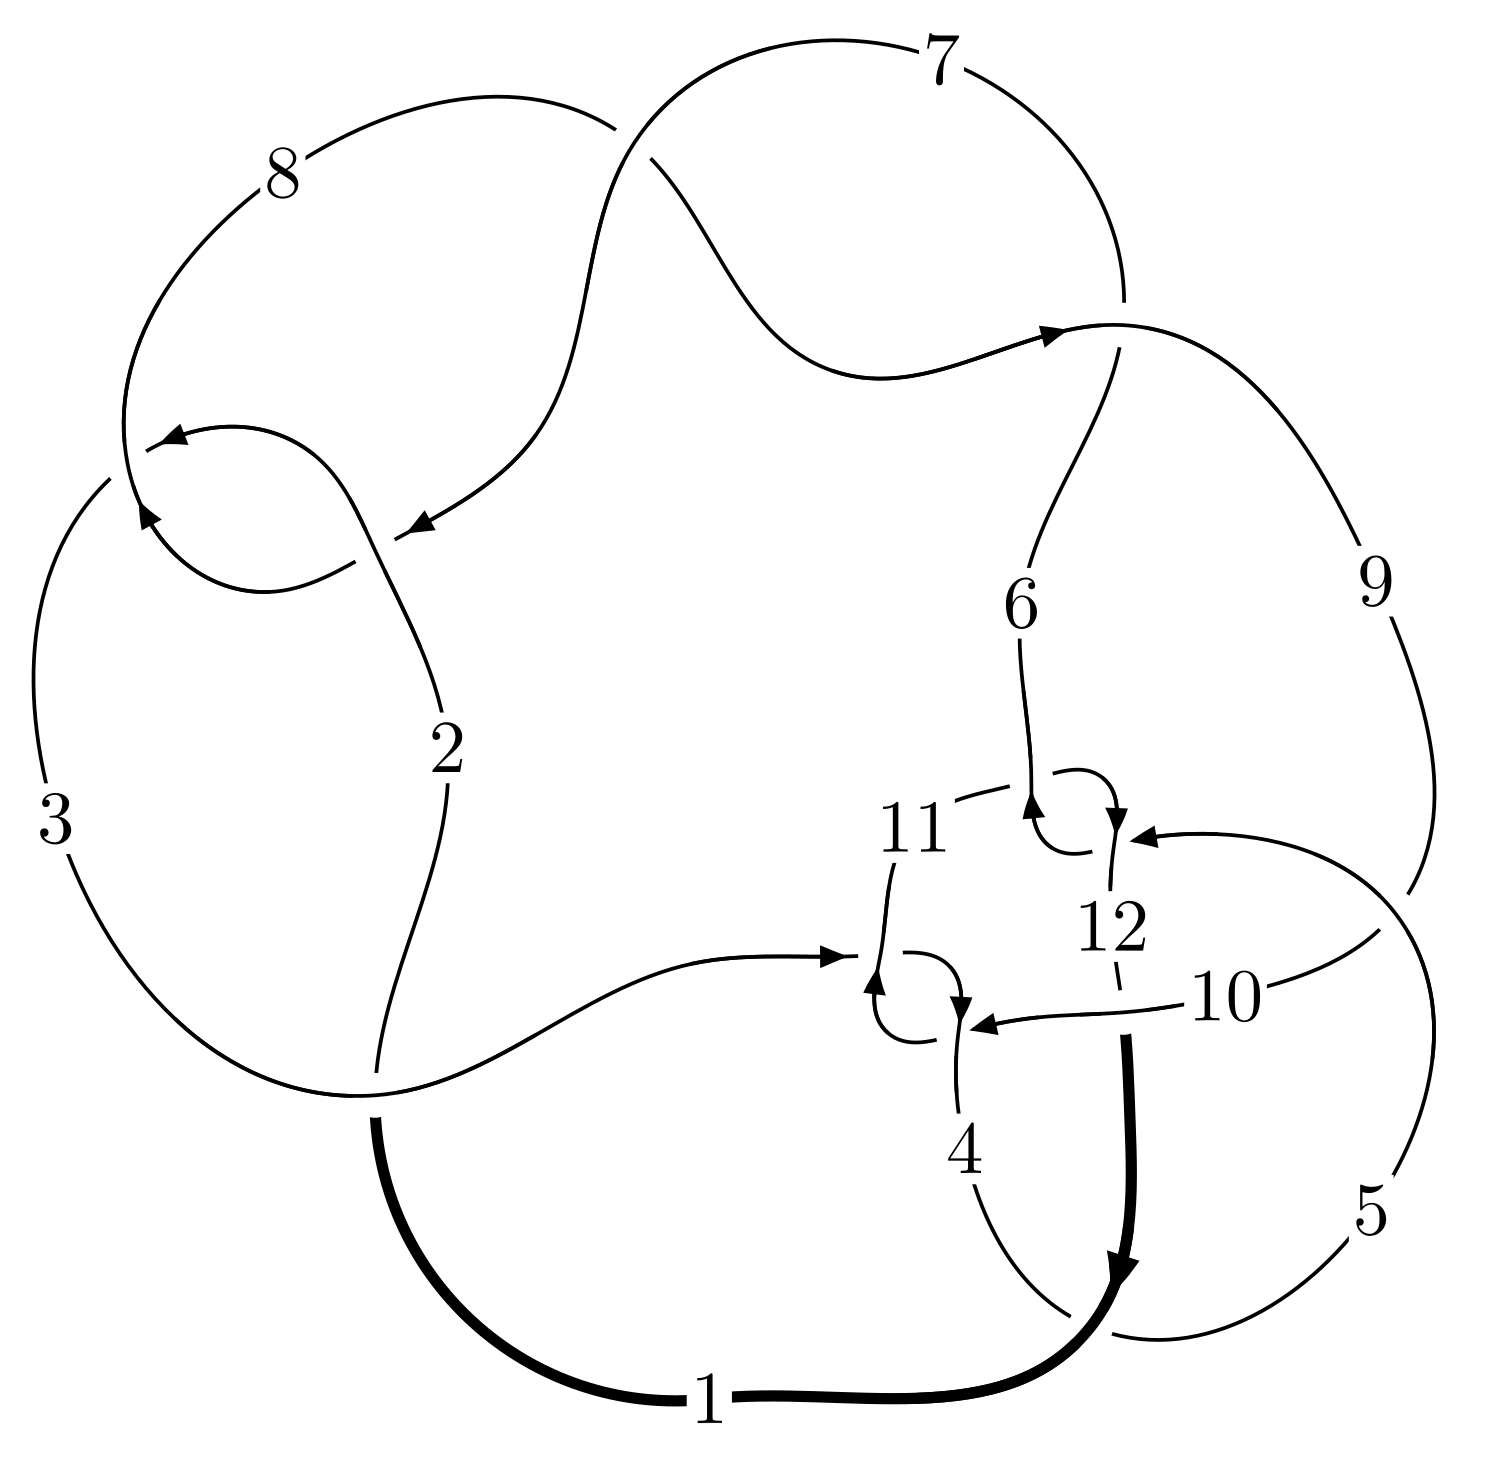
\includegraphics[width=112pt]{../../../GIT/diagram.site/Diagrams/png/1600_12a_0799.png}\\
\ \ \ A knot diagram\footnotemark}&
\allowdisplaybreaks
\textbf{Linearized knot diagam} \\
\cline{2-2}
 &
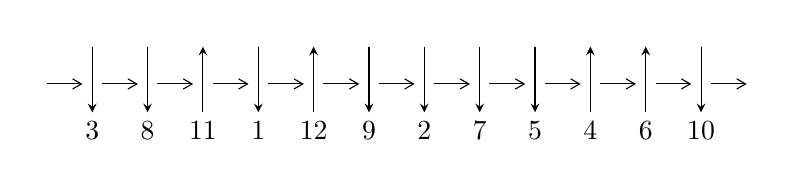
\begin{tikzpicture}[x=20pt, y=17pt]
	% nodes
	\node (C0) at (0, 0) {};
	\node (C1) at (1, 0) {};
	\node (C1U) at (1, +1) {};
	\node (C1D) at (1, -1) {3};

	\node (C2) at (2, 0) {};
	\node (C2U) at (2, +1) {};
	\node (C2D) at (2, -1) {8};

	\node (C3) at (3, 0) {};
	\node (C3U) at (3, +1) {};
	\node (C3D) at (3, -1) {11};

	\node (C4) at (4, 0) {};
	\node (C4U) at (4, +1) {};
	\node (C4D) at (4, -1) {1};

	\node (C5) at (5, 0) {};
	\node (C5U) at (5, +1) {};
	\node (C5D) at (5, -1) {12};

	\node (C6) at (6, 0) {};
	\node (C6U) at (6, +1) {};
	\node (C6D) at (6, -1) {9};

	\node (C7) at (7, 0) {};
	\node (C7U) at (7, +1) {};
	\node (C7D) at (7, -1) {2};

	\node (C8) at (8, 0) {};
	\node (C8U) at (8, +1) {};
	\node (C8D) at (8, -1) {7};

	\node (C9) at (9, 0) {};
	\node (C9U) at (9, +1) {};
	\node (C9D) at (9, -1) {5};

	\node (C10) at (10, 0) {};
	\node (C10U) at (10, +1) {};
	\node (C10D) at (10, -1) {4};

	\node (C11) at (11, 0) {};
	\node (C11U) at (11, +1) {};
	\node (C11D) at (11, -1) {6};

	\node (C12) at (12, 0) {};
	\node (C12U) at (12, +1) {};
	\node (C12D) at (12, -1) {10};
	\node (C13) at (13, 0) {};

	% arrows
	\draw[->,>={angle 60}]
	(C0) edge (C1) (C1) edge (C2) (C2) edge (C3) (C3) edge (C4) (C4) edge (C5) (C5) edge (C6) (C6) edge (C7) (C7) edge (C8) (C8) edge (C9) (C9) edge (C10) (C10) edge (C11) (C11) edge (C12) (C12) edge (C13) ;	\draw[->,>=stealth]
	(C1U) edge (C1D) (C2U) edge (C2D) (C3D) edge (C3U) (C4U) edge (C4D) (C5D) edge (C5U) (C6U) edge (C6D) (C7U) edge (C7D) (C8U) edge (C8D) (C9U) edge (C9D) (C10D) edge (C10U) (C11D) edge (C11U) (C12U) edge (C12D) ;
	\end{tikzpicture} \\
\hhline{~~} \\& 
\textbf{Solving Sequence} \\ \cline{2-2} 
 &
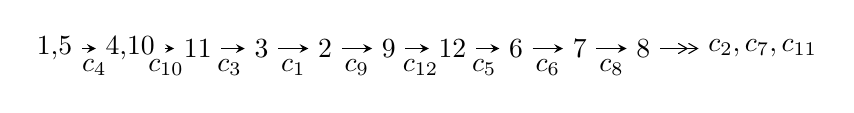
\begin{tikzpicture}[x=23pt, y=7pt]
	% node
	\node (A0) at (-1/8, 0) {1,5};
	\node (A1) at (17/16, 0) {4,10};
	\node (A2) at (17/8, 0) {11};
	\node (A3) at (25/8, 0) {3};
	\node (A4) at (33/8, 0) {2};
	\node (A5) at (41/8, 0) {9};
	\node (A6) at (49/8, 0) {12};
	\node (A7) at (57/8, 0) {6};
	\node (A8) at (65/8, 0) {7};
	\node (A9) at (73/8, 0) {8};
	\node (C1) at (1/2, -1) {$c_{4}$};
	\node (C2) at (13/8, -1) {$c_{10}$};
	\node (C3) at (21/8, -1) {$c_{3}$};
	\node (C4) at (29/8, -1) {$c_{1}$};
	\node (C5) at (37/8, -1) {$c_{9}$};
	\node (C6) at (45/8, -1) {$c_{12}$};
	\node (C7) at (53/8, -1) {$c_{5}$};
	\node (C8) at (61/8, -1) {$c_{6}$};
	\node (C9) at (69/8, -1) {$c_{8}$};
	\node (A10) at (11, 0) {$c_{2},c_{7},c_{11}$};

	% edge
	\draw[->,>=stealth]	
	(A0) edge (A1) (A1) edge (A2) (A2) edge (A3) (A3) edge (A4) (A4) edge (A5) (A5) edge (A6) (A6) edge (A7) (A7) edge (A8) (A8) edge (A9) ;
	\draw[->>,>={angle 60}]	
	(A9) edge (A10);
\end{tikzpicture} \\ 

\end{tabular} \\

\footnotetext{
The image of knot diagram is generated by the software ``\textbf{Draw programme}" developed by Andrew Bartholomew(\url{http://www.layer8.co.uk/maths/draw/index.htm\#Running-draw}), where we modified some parts for our purpose(\url{https://github.com/CATsTAILs/LinksPainter}).
}\phantom \\ \newline 
\centering \textbf{Ideals for irreducible components\footnotemark of $X_{\text{par}}$} 
 
\begin{align*}
I^u_{1}&=\langle 
b- u,\;-4.30859\times10^{43} u^{34}-5.23230\times10^{43} u^{33}+\cdots+2.27410\times10^{43} a+1.99881\times10^{44},\\
\phantom{I^u_{1}}&\phantom{= \langle  }u^{35}+u^{34}+\cdots-2 u-1\rangle \\
I^u_{2}&=\langle 
1.34503\times10^{309} u^{71}+4.07190\times10^{309} u^{70}+\cdots+3.30547\times10^{309} b+2.52151\times10^{310},\\
\phantom{I^u_{2}}&\phantom{= \langle  }-2.10209\times10^{240} u^{71}-6.36722\times10^{240} u^{70}+\cdots+3.89663\times10^{240} a-1.36055\times10^{242},\\
\phantom{I^u_{2}}&\phantom{= \langle  }u^{72}+3 u^{71}+\cdots+48 u+1\rangle \\
I^u_{3}&=\langle 
b+u,\;-886 u^{19}-1725 u^{18}+\cdots+2249 a+1906,\;u^{20}+u^{19}+\cdots-2 u+1\rangle \\
\\
\end{align*}
\raggedright * 3 irreducible components of $\dim_{\mathbb{C}}=0$, with total 127 representations.\\
\footnotetext{All coefficients of polynomials are rational numbers. But the coefficients are sometimes approximated in decimal forms when there is not enough margin.}
\newpage
\renewcommand{\arraystretch}{1}
\centering \section*{I. $I^u_{1}= \langle b- u,\;-4.31\times10^{43} u^{34}-5.23\times10^{43} u^{33}+\cdots+2.27\times10^{43} a+2.00\times10^{44},\;u^{35}+u^{34}+\cdots-2 u-1 \rangle$}
\flushleft \textbf{(i) Arc colorings}\\
\begin{tabular}{m{7pt} m{180pt} m{7pt} m{180pt} }
\flushright $a_{1}=$&$\begin{pmatrix}0\\u\end{pmatrix}$ \\
\flushright $a_{5}=$&$\begin{pmatrix}1\\0\end{pmatrix}$ \\
\flushright $a_{4}=$&$\begin{pmatrix}1\\- u^2\end{pmatrix}$ \\
\flushright $a_{10}=$&$\begin{pmatrix}1.89464 u^{34}+2.30083 u^{33}+\cdots-29.6286 u-8.78949\\u\end{pmatrix}$ \\
\flushright $a_{11}=$&$\begin{pmatrix}1.95202 u^{34}+2.28719 u^{33}+\cdots-25.9216 u-8.38330\\0.0586830 u^{34}+0.0132193 u^{33}+\cdots+1.08465 u+0.0710140\end{pmatrix}$ \\
\flushright $a_{3}=$&$\begin{pmatrix}1.63631 u^{34}+1.06267 u^{33}+\cdots-17.1111 u+4.79896\\-0.136168 u^{34}-0.222641 u^{33}+\cdots+0.865605 u+0.173572\end{pmatrix}$ \\
\flushright $a_{2}=$&$\begin{pmatrix}0.267879 u^{34}+1.37848 u^{33}+\cdots-3.97515 u-10.7436\\-0.167035 u^{34}-0.151989 u^{33}+\cdots+3.05890 u+0.326704\end{pmatrix}$ \\
\flushright $a_{9}=$&$\begin{pmatrix}1.89464 u^{34}+2.30083 u^{33}+\cdots-28.6286 u-8.78949\\u\end{pmatrix}$ \\
\flushright $a_{12}=$&$\begin{pmatrix}2.30439 u^{34}+3.64678 u^{33}+\cdots-19.4192 u-18.0743\\0.0573800 u^{34}-0.0136340 u^{33}+\cdots+3.70702 u+0.406189\end{pmatrix}$ \\
\flushright $a_{6}=$&$\begin{pmatrix}-4.47995 u^{34}-3.38545 u^{33}+\cdots+40.8417 u+3.13769\\0.112272 u^{34}+0.228464 u^{33}+\cdots-1.35463 u+0.400070\end{pmatrix}$ \\
\flushright $a_{7}=$&$\begin{pmatrix}0.207182 u^{34}+0.352338 u^{33}+\cdots-1.38655 u+0.769048\\0.136168 u^{34}+0.222641 u^{33}+\cdots-0.865605 u-0.173572\end{pmatrix}$ \\
\flushright $a_{8}=$&$\begin{pmatrix}1.04114 u^{34}+1.50676 u^{33}+\cdots-16.4681 u-6.55811\\-0.167035 u^{34}-0.151989 u^{33}+\cdots+3.05890 u+0.326704\end{pmatrix}$\\&\end{tabular}
\flushleft \textbf{(ii) Obstruction class $= -1$}\\~\\
\flushleft \textbf{(iii) Cusp Shapes $= -8.40302 u^{34}-4.98573 u^{33}+\cdots+50.7095 u-6.32050$}\\~\\
\newpage\renewcommand{\arraystretch}{1}
\flushleft \textbf{(iv) u-Polynomials at the component}\newline \\
\begin{tabular}{m{50pt}|m{274pt}}
Crossings & \hspace{64pt}u-Polynomials at each crossing \\
\hline $$\begin{aligned}c_{1},c_{6},c_{8}\end{aligned}$$&$\begin{aligned}
&u^{35}+9 u^{34}+\cdots+16 u+64
\end{aligned}$\\
\hline $$\begin{aligned}c_{2},c_{7}\end{aligned}$$&$\begin{aligned}
&u^{35}+7 u^{34}+\cdots+20 u+8
\end{aligned}$\\
\hline $$\begin{aligned}c_{3},c_{5},c_{10}\\c_{11}\end{aligned}$$&$\begin{aligned}
&u^{35}+10 u^{33}+\cdots+3 u+1
\end{aligned}$\\
\hline $$\begin{aligned}c_{4},c_{9}\end{aligned}$$&$\begin{aligned}
&u^{35}- u^{34}+\cdots-2 u+1
\end{aligned}$\\
\hline $$\begin{aligned}c_{12}\end{aligned}$$&$\begin{aligned}
&u^{35}-27 u^{34}+\cdots+73728 u-4096
\end{aligned}$\\
\hline
\end{tabular}\\~\\
\newpage\renewcommand{\arraystretch}{1}
\flushleft \textbf{(v) Riley Polynomials at the component}\newline \\
\begin{tabular}{m{50pt}|m{274pt}}
Crossings & \hspace{64pt}Riley Polynomials at each crossing \\
\hline $$\begin{aligned}c_{1},c_{6},c_{8}\end{aligned}$$&$\begin{aligned}
&y^{35}+35 y^{34}+\cdots+34048 y-4096
\end{aligned}$\\
\hline $$\begin{aligned}c_{2},c_{7}\end{aligned}$$&$\begin{aligned}
&y^{35}-9 y^{34}+\cdots+16 y-64
\end{aligned}$\\
\hline $$\begin{aligned}c_{3},c_{5},c_{10}\\c_{11}\end{aligned}$$&$\begin{aligned}
&y^{35}+20 y^{34}+\cdots+y-1
\end{aligned}$\\
\hline $$\begin{aligned}c_{4},c_{9}\end{aligned}$$&$\begin{aligned}
&y^{35}+15 y^{34}+\cdots-34 y-1
\end{aligned}$\\
\hline $$\begin{aligned}c_{12}\end{aligned}$$&$\begin{aligned}
&y^{35}-11 y^{34}+\cdots+125829120 y-16777216
\end{aligned}$\\
\hline
\end{tabular}\\~\\
\newpage\flushleft \textbf{(vi) Complex Volumes and Cusp Shapes}
$$\begin{array}{c|c|c}  
\text{Solutions to }I^u_{1}& \I (\text{vol} + \sqrt{-1}CS) & \text{Cusp shape}\\
 \hline 
\begin{aligned}
u &= \phantom{-}0.591089 + 0.775481 I \\
a &= -0.687556 + 0.152845 I \\
b &= \phantom{-}0.591089 + 0.775481 I\end{aligned}
 & \phantom{-}1.33872 - 3.31510 I & \phantom{-}0.58501 + 5.76749 I \\ \hline\begin{aligned}
u &= \phantom{-}0.591089 - 0.775481 I \\
a &= -0.687556 - 0.152845 I \\
b &= \phantom{-}0.591089 - 0.775481 I\end{aligned}
 & \phantom{-}1.33872 + 3.31510 I & \phantom{-}0.58501 - 5.76749 I \\ \hline\begin{aligned}
u &= -0.597092 + 0.966307 I \\
a &= \phantom{-}1.29984 + 0.98350 I \\
b &= -0.597092 + 0.966307 I\end{aligned}
 & -3.80954 - 0.35655 I & -7.72758 - 2.31082 I \\ \hline\begin{aligned}
u &= -0.597092 - 0.966307 I \\
a &= \phantom{-}1.29984 - 0.98350 I \\
b &= -0.597092 - 0.966307 I\end{aligned}
 & -3.80954 + 0.35655 I & -7.72758 + 2.31082 I \\ \hline\begin{aligned}
u &= -0.274359 + 0.767854 I \\
a &= \phantom{-}0.872835 + 0.188368 I \\
b &= -0.274359 + 0.767854 I\end{aligned}
 & \phantom{-}2.17204 - 0.64743 I & \phantom{-}3.30372 + 2.66194 I \\ \hline\begin{aligned}
u &= -0.274359 - 0.767854 I \\
a &= \phantom{-}0.872835 - 0.188368 I \\
b &= -0.274359 - 0.767854 I\end{aligned}
 & \phantom{-}2.17204 + 0.64743 I & \phantom{-}3.30372 - 2.66194 I \\ \hline\begin{aligned}
u &= -0.413251 + 1.183840 I \\
a &= \phantom{-}0.674185 + 0.327128 I \\
b &= -0.413251 + 1.183840 I\end{aligned}
 & \phantom{-}9.66329 - 0.96587 I & \phantom{-}3.05582 + 0.39367 I \\ \hline\begin{aligned}
u &= -0.413251 - 1.183840 I \\
a &= \phantom{-}0.674185 - 0.327128 I \\
b &= -0.413251 - 1.183840 I\end{aligned}
 & \phantom{-}9.66329 + 0.96587 I & \phantom{-}3.05582 - 0.39367 I \\ \hline\begin{aligned}
u &= \phantom{-}0.419219 + 0.615155 I \\
a &= \phantom{-}1.22242 + 1.49117 I \\
b &= \phantom{-}0.419219 + 0.615155 I\end{aligned}
 & \phantom{-}5.07676 - 3.71447 I & -0.77708 + 4.68220 I \\ \hline\begin{aligned}
u &= \phantom{-}0.419219 - 0.615155 I \\
a &= \phantom{-}1.22242 - 1.49117 I \\
b &= \phantom{-}0.419219 - 0.615155 I\end{aligned}
 & \phantom{-}5.07676 + 3.71447 I & -0.77708 - 4.68220 I\\
 \hline 
 \end{array}$$\newpage$$\begin{array}{c|c|c}  
\text{Solutions to }I^u_{1}& \I (\text{vol} + \sqrt{-1}CS) & \text{Cusp shape}\\
 \hline 
\begin{aligned}
u &= -0.466745 + 0.574137 I \\
a &= -1.13727 + 1.70318 I \\
b &= -0.466745 + 0.574137 I\end{aligned}
 & \phantom{-}4.38894 + 9.97061 I & -2.42520 - 9.73459 I \\ \hline\begin{aligned}
u &= -0.466745 - 0.574137 I \\
a &= -1.13727 - 1.70318 I \\
b &= -0.466745 - 0.574137 I\end{aligned}
 & \phantom{-}4.38894 - 9.97061 I & -2.42520 + 9.73459 I \\ \hline\begin{aligned}
u &= \phantom{-}0.474572 + 1.194770 I \\
a &= -0.658032 + 0.313634 I \\
b &= \phantom{-}0.474572 + 1.194770 I\end{aligned}
 & \phantom{-}9.55181 - 5.46707 I & \phantom{-}2.92000 + 4.74682 I \\ \hline\begin{aligned}
u &= \phantom{-}0.474572 - 1.194770 I \\
a &= -0.658032 - 0.313634 I \\
b &= \phantom{-}0.474572 - 1.194770 I\end{aligned}
 & \phantom{-}9.55181 + 5.46707 I & \phantom{-}2.92000 - 4.74682 I \\ \hline\begin{aligned}
u &= \phantom{-}0.723524 + 1.111440 I \\
a &= -1.045310 + 0.708906 I \\
b &= \phantom{-}0.723524 + 1.111440 I\end{aligned}
 & -2.05608 - 5.08661 I & -4.00000 + 6.93227 I \\ \hline\begin{aligned}
u &= \phantom{-}0.723524 - 1.111440 I \\
a &= -1.045310 - 0.708906 I \\
b &= \phantom{-}0.723524 - 1.111440 I\end{aligned}
 & -2.05608 + 5.08661 I & -4.00000 - 6.93227 I \\ \hline\begin{aligned}
u &= -0.950167 + 0.965088 I \\
a &= \phantom{-}1.212470 + 0.335142 I \\
b &= -0.950167 + 0.965088 I\end{aligned}
 & -8.23917 + 6.19708 I & -11.53177 - 4.77423 I \\ \hline\begin{aligned}
u &= -0.950167 - 0.965088 I \\
a &= \phantom{-}1.212470 - 0.335142 I \\
b &= -0.950167 - 0.965088 I\end{aligned}
 & -8.23917 - 6.19708 I & -11.53177 + 4.77423 I \\ \hline\begin{aligned}
u &= \phantom{-}0.597400\phantom{ +0.000000I} \\
a &= -0.567434\phantom{ +0.000000I} \\
b &= \phantom{-}0.597400\phantom{ +0.000000I}\end{aligned}
 & -1.22075\phantom{ +0.000000I} & -7.22590\phantom{ +0.000000I} \\ \hline\begin{aligned}
u &= \phantom{-}0.097938 + 0.514145 I \\
a &= \phantom{-}1.96245 + 0.19680 I \\
b &= \phantom{-}0.097938 + 0.514145 I\end{aligned}
 & \phantom{-}0.44134 - 1.63347 I & \phantom{-}1.73800 + 4.33093 I\\
 \hline 
 \end{array}$$\newpage$$\begin{array}{c|c|c}  
\text{Solutions to }I^u_{1}& \I (\text{vol} + \sqrt{-1}CS) & \text{Cusp shape}\\
 \hline 
\begin{aligned}
u &= \phantom{-}0.097938 - 0.514145 I \\
a &= \phantom{-}1.96245 - 0.19680 I \\
b &= \phantom{-}0.097938 - 0.514145 I\end{aligned}
 & \phantom{-}0.44134 + 1.63347 I & \phantom{-}1.73800 - 4.33093 I \\ \hline\begin{aligned}
u &= -0.271525 + 0.415826 I \\
a &= -2.75306 + 1.67750 I \\
b &= -0.271525 + 0.415826 I\end{aligned}
 & -2.74916 + 4.77966 I & -3.72482 - 10.00221 I \\ \hline\begin{aligned}
u &= -0.271525 - 0.415826 I \\
a &= -2.75306 - 1.67750 I \\
b &= -0.271525 - 0.415826 I\end{aligned}
 & -2.74916 - 4.77966 I & -3.72482 + 10.00221 I \\ \hline\begin{aligned}
u &= \phantom{-}1.03004 + 1.11959 I \\
a &= -0.999328 + 0.306692 I \\
b &= \phantom{-}1.03004 + 1.11959 I\end{aligned}
 & -3.63302 - 8.69335 I & \phantom{-0.000000 } 0 \\ \hline\begin{aligned}
u &= \phantom{-}1.03004 - 1.11959 I \\
a &= -0.999328 - 0.306692 I \\
b &= \phantom{-}1.03004 - 1.11959 I\end{aligned}
 & -3.63302 + 8.69335 I & \phantom{-0.000000 } 0 \\ \hline\begin{aligned}
u &= \phantom{-}0.06773 + 1.55270 I \\
a &= -0.068133 + 0.960500 I \\
b &= \phantom{-}0.06773 + 1.55270 I\end{aligned}
 & \phantom{-}8.19666 - 3.43452 I & \phantom{-0.000000 } 0 \\ \hline\begin{aligned}
u &= \phantom{-}0.06773 - 1.55270 I \\
a &= -0.068133 - 0.960500 I \\
b &= \phantom{-}0.06773 - 1.55270 I\end{aligned}
 & \phantom{-}8.19666 + 3.43452 I & \phantom{-0.000000 } 0 \\ \hline\begin{aligned}
u &= -1.13426 + 1.07638 I \\
a &= \phantom{-}1.002730 + 0.193039 I \\
b &= -1.13426 + 1.07638 I\end{aligned}
 & -6.3568 + 12.9060 I & \phantom{-0.000000 } 0 \\ \hline\begin{aligned}
u &= -1.13426 - 1.07638 I \\
a &= \phantom{-}1.002730 - 0.193039 I \\
b &= -1.13426 - 1.07638 I\end{aligned}
 & -6.3568 - 12.9060 I & \phantom{-0.000000 } 0 \\ \hline\begin{aligned}
u &= -0.067600 + 0.311475 I \\
a &= -3.61790 - 2.90700 I \\
b &= -0.067600 + 0.311475 I\end{aligned}
 & -2.02184 - 1.48778 I & -5.29371 + 6.36546 I\\
 \hline 
 \end{array}$$\newpage$$\begin{array}{c|c|c}  
\text{Solutions to }I^u_{1}& \I (\text{vol} + \sqrt{-1}CS) & \text{Cusp shape}\\
 \hline 
\begin{aligned}
u &= -0.067600 - 0.311475 I \\
a &= -3.61790 + 2.90700 I \\
b &= -0.067600 - 0.311475 I\end{aligned}
 & -2.02184 + 1.48778 I & -5.29371 - 6.36546 I \\ \hline\begin{aligned}
u &= \phantom{-}1.20419 + 1.21154 I \\
a &= -0.874512 + 0.183122 I \\
b &= \phantom{-}1.20419 + 1.21154 I\end{aligned}
 & \phantom{-}2.43884 - 11.28800 I & \phantom{-0.000000 } 0 \\ \hline\begin{aligned}
u &= \phantom{-}1.20419 - 1.21154 I \\
a &= -0.874512 - 0.183122 I \\
b &= \phantom{-}1.20419 - 1.21154 I\end{aligned}
 & \phantom{-}2.43884 + 11.28800 I & \phantom{-0.000000 } 0 \\ \hline\begin{aligned}
u &= -1.23200 + 1.19581 I \\
a &= \phantom{-}0.877886 + 0.159904 I \\
b &= -1.23200 + 1.19581 I\end{aligned}
 & \phantom{-}1.8345 + 17.7184 I & \phantom{-0.000000 } 0 \\ \hline\begin{aligned}
u &= -1.23200 - 1.19581 I \\
a &= \phantom{-}0.877886 - 0.159904 I \\
b &= -1.23200 - 1.19581 I\end{aligned}
 & \phantom{-}1.8345 - 17.7184 I & \phantom{-0.000000 } 0\\
 \hline 
 \end{array}$$\newpage\newpage\renewcommand{\arraystretch}{1}
\centering \section*{II. $I^u_{2}= \langle 1.35\times10^{309} u^{71}+4.07\times10^{309} u^{70}+\cdots+3.31\times10^{309} b+2.52\times10^{310},\;-2.10\times10^{240} u^{71}-6.37\times10^{240} u^{70}+\cdots+3.90\times10^{240} a-1.36\times10^{242},\;u^{72}+3 u^{71}+\cdots+48 u+1 \rangle$}
\flushleft \textbf{(i) Arc colorings}\\
\begin{tabular}{m{7pt} m{180pt} m{7pt} m{180pt} }
\flushright $a_{1}=$&$\begin{pmatrix}0\\u\end{pmatrix}$ \\
\flushright $a_{5}=$&$\begin{pmatrix}1\\0\end{pmatrix}$ \\
\flushright $a_{4}=$&$\begin{pmatrix}1\\- u^2\end{pmatrix}$ \\
\flushright $a_{10}=$&$\begin{pmatrix}0.539465 u^{71}+1.63403 u^{70}+\cdots+603.712 u+34.9160\\-0.406910 u^{71}-1.23187 u^{70}+\cdots-242.608 u-7.62829\end{pmatrix}$ \\
\flushright $a_{11}=$&$\begin{pmatrix}0.135898 u^{71}+0.410976 u^{70}+\cdots+359.814 u+27.2721\\-0.433293 u^{71}-1.29628 u^{70}+\cdots-243.604 u-7.64065\end{pmatrix}$ \\
\flushright $a_{3}=$&$\begin{pmatrix}-5.47361 u^{71}-15.9771 u^{70}+\cdots-3245.98 u-92.7647\\0.0926148 u^{71}+0.257322 u^{70}+\cdots+41.1552 u-2.78210\end{pmatrix}$ \\
\flushright $a_{2}=$&$\begin{pmatrix}-0.130468 u^{71}-0.583660 u^{70}+\cdots-769.572 u-70.4281\\1.03009 u^{71}+3.02070 u^{70}+\cdots+634.312 u+21.1555\end{pmatrix}$ \\
\flushright $a_{9}=$&$\begin{pmatrix}0.132555 u^{71}+0.402165 u^{70}+\cdots+361.104 u+27.2877\\-0.406910 u^{71}-1.23187 u^{70}+\cdots-242.608 u-7.62829\end{pmatrix}$ \\
\flushright $a_{12}=$&$\begin{pmatrix}-0.232683 u^{71}-0.798062 u^{70}+\cdots-461.851 u-26.5601\\0.400276 u^{71}+1.09127 u^{70}+\cdots+167.198 u+5.35353\end{pmatrix}$ \\
\flushright $a_{6}=$&$\begin{pmatrix}4.24388 u^{71}+12.1560 u^{70}+\cdots+1995.98 u+55.1998\\-0.237755 u^{71}-0.677729 u^{70}+\cdots-47.8013 u+1.19648\end{pmatrix}$ \\
\flushright $a_{7}=$&$\begin{pmatrix}7.24447 u^{71}+21.3193 u^{70}+\cdots+4321.80 u+124.943\\-0.396176 u^{71}-1.16932 u^{70}+\cdots-127.116 u+1.79571\end{pmatrix}$ \\
\flushright $a_{8}=$&$\begin{pmatrix}0.727709 u^{71}+1.96306 u^{70}+\cdots-275.156 u-53.7910\\0.803345 u^{71}+2.34508 u^{70}+\cdots+560.708 u+19.6459\end{pmatrix}$\\&\end{tabular}
\flushleft \textbf{(ii) Obstruction class $= -1$}\\~\\
\flushleft \textbf{(iii) Cusp Shapes $= -0.619107 u^{71}-1.70406 u^{70}+\cdots+144.641 u-5.48872$}\\~\\
\newpage\renewcommand{\arraystretch}{1}
\flushleft \textbf{(iv) u-Polynomials at the component}\newline \\
\begin{tabular}{m{50pt}|m{274pt}}
Crossings & \hspace{64pt}u-Polynomials at each crossing \\
\hline $$\begin{aligned}c_{1},c_{6},c_{8}\end{aligned}$$&$\begin{aligned}
&(u^{12}+3 u^{11}+\cdots+2 u+1)^{6}
\end{aligned}$\\
\hline $$\begin{aligned}c_{2},c_{7}\end{aligned}$$&$\begin{aligned}
&(u^{12}- u^{11}- u^{10}+2 u^9+3 u^8-4 u^7-2 u^6+4 u^5+2 u^4-3 u^3- u^2+1)^6
\end{aligned}$\\
\hline $$\begin{aligned}c_{3},c_{5},c_{10}\\c_{11}\end{aligned}$$&$\begin{aligned}
&u^{72}- u^{71}+\cdots+13014 u+2943
\end{aligned}$\\
\hline $$\begin{aligned}c_{4},c_{9}\end{aligned}$$&$\begin{aligned}
&u^{72}-3 u^{71}+\cdots-48 u+1
\end{aligned}$\\
\hline $$\begin{aligned}c_{12}\end{aligned}$$&$\begin{aligned}
&(u^3+u^2-1)^{24}
\end{aligned}$\\
\hline
\end{tabular}\\~\\
\newpage\renewcommand{\arraystretch}{1}
\flushleft \textbf{(v) Riley Polynomials at the component}\newline \\
\begin{tabular}{m{50pt}|m{274pt}}
Crossings & \hspace{64pt}Riley Polynomials at each crossing \\
\hline $$\begin{aligned}c_{1},c_{6},c_{8}\end{aligned}$$&$\begin{aligned}
&(y^{12}+13 y^{11}+\cdots+6 y+1)^{6}
\end{aligned}$\\
\hline $$\begin{aligned}c_{2},c_{7}\end{aligned}$$&$\begin{aligned}
&(y^{12}-3 y^{11}+\cdots-2 y+1)^{6}
\end{aligned}$\\
\hline $$\begin{aligned}c_{3},c_{5},c_{10}\\c_{11}\end{aligned}$$&$\begin{aligned}
&y^{72}+51 y^{71}+\cdots+376303320 y+8661249
\end{aligned}$\\
\hline $$\begin{aligned}c_{4},c_{9}\end{aligned}$$&$\begin{aligned}
&y^{72}-17 y^{71}+\cdots-552 y+1
\end{aligned}$\\
\hline $$\begin{aligned}c_{12}\end{aligned}$$&$\begin{aligned}
&(y^3- y^2+2 y-1)^{24}
\end{aligned}$\\
\hline
\end{tabular}\\~\\
\newpage\flushleft \textbf{(vi) Complex Volumes and Cusp Shapes}
$$\begin{array}{c|c|c}  
\text{Solutions to }I^u_{2}& \I (\text{vol} + \sqrt{-1}CS) & \text{Cusp shape}\\
 \hline 
\begin{aligned}
u &= -0.568176 + 0.839836 I \\
a &= -1.093330 - 0.305104 I \\
b &= \phantom{-}1.23118 - 1.38930 I\end{aligned}
 & \phantom{-}6.00451 + 4.31046 I & \phantom{-0.000000 } 0 \\ \hline\begin{aligned}
u &= -0.568176 - 0.839836 I \\
a &= -1.093330 + 0.305104 I \\
b &= \phantom{-}1.23118 + 1.38930 I\end{aligned}
 & \phantom{-}6.00451 - 4.31046 I & \phantom{-0.000000 } 0 \\ \hline\begin{aligned}
u &= \phantom{-}0.891554 + 0.489577 I \\
a &= \phantom{-}1.108640 + 0.226678 I \\
b &= -1.30602 - 0.59539 I\end{aligned}
 & -3.34798 - 2.47502 I & \phantom{-0.000000 } 0 \\ \hline\begin{aligned}
u &= \phantom{-}0.891554 - 0.489577 I \\
a &= \phantom{-}1.108640 - 0.226678 I \\
b &= -1.30602 + 0.59539 I\end{aligned}
 & -3.34798 + 2.47502 I & \phantom{-0.000000 } 0 \\ \hline\begin{aligned}
u &= \phantom{-}0.701909 + 0.683885 I \\
a &= \phantom{-}1.171710 - 0.080430 I \\
b &= -1.28434 - 1.06706 I\end{aligned}
 & -1.98742 - 7.07733 I & \phantom{-0.000000 } 0 \\ \hline\begin{aligned}
u &= \phantom{-}0.701909 - 0.683885 I \\
a &= \phantom{-}1.171710 + 0.080430 I \\
b &= -1.28434 + 1.06706 I\end{aligned}
 & -1.98742 + 7.07733 I & \phantom{-0.000000 } 0 \\ \hline\begin{aligned}
u &= \phantom{-}0.977106 + 0.046716 I \\
a &= \phantom{-}0.859586 - 0.803411 I \\
b &= -0.875721 + 0.368859 I\end{aligned}
 & -3.34798 + 3.18123 I & \phantom{-0.000000 } 0 \\ \hline\begin{aligned}
u &= \phantom{-}0.977106 - 0.046716 I \\
a &= \phantom{-}0.859586 + 0.803411 I \\
b &= -0.875721 - 0.368859 I\end{aligned}
 & -3.34798 - 3.18123 I & \phantom{-0.000000 } 0 \\ \hline\begin{aligned}
u &= \phantom{-}0.604256 + 0.853075 I \\
a &= \phantom{-}1.066580 - 0.273076 I \\
b &= -1.29161 - 1.38021 I\end{aligned}
 & \phantom{-}5.64748 - 10.62950 I & \phantom{-0.000000 } 0 \\ \hline\begin{aligned}
u &= \phantom{-}0.604256 - 0.853075 I \\
a &= \phantom{-}1.066580 + 0.273076 I \\
b &= -1.29161 + 1.38021 I\end{aligned}
 & \phantom{-}5.64748 + 10.62950 I & \phantom{-0.000000 } 0\\
 \hline 
 \end{array}$$\newpage$$\begin{array}{c|c|c}  
\text{Solutions to }I^u_{2}& \I (\text{vol} + \sqrt{-1}CS) & \text{Cusp shape}\\
 \hline 
\begin{aligned}
u &= \phantom{-}0.509449 + 0.806111 I \\
a &= \phantom{-}1.151870 - 0.360525 I \\
b &= -0.302346 - 0.194987 I\end{aligned}
 & -0.17094 - 2.11219 I & \phantom{-0.000000 } 0 \\ \hline\begin{aligned}
u &= \phantom{-}0.509449 - 0.806111 I \\
a &= \phantom{-}1.151870 + 0.360525 I \\
b &= -0.302346 + 0.194987 I\end{aligned}
 & -0.17094 + 2.11219 I & \phantom{-0.000000 } 0 \\ \hline\begin{aligned}
u &= -0.875721 + 0.368859 I \\
a &= -1.155270 + 0.363964 I \\
b &= \phantom{-}0.977106 + 0.046716 I\end{aligned}
 & -3.34798 + 3.18123 I & \phantom{-0.000000 } 0 \\ \hline\begin{aligned}
u &= -0.875721 - 0.368859 I \\
a &= -1.155270 - 0.363964 I \\
b &= \phantom{-}0.977106 - 0.046716 I\end{aligned}
 & -3.34798 - 3.18123 I & \phantom{-0.000000 } 0 \\ \hline\begin{aligned}
u &= -0.904826 + 0.206753 I \\
a &= \phantom{-}0.792882 + 0.181173 I \\
b &= -1.32231 - 1.27743 I\end{aligned}
 & -6.12500 + 4.24921 I & -13.1960 - 6.9831 I \\ \hline\begin{aligned}
u &= -0.904826 - 0.206753 I \\
a &= \phantom{-}0.792882 - 0.181173 I \\
b &= -1.32231 + 1.27743 I\end{aligned}
 & -6.12500 - 4.24921 I & -13.1960 + 6.9831 I \\ \hline\begin{aligned}
u &= \phantom{-}1.013100 + 0.432835 I \\
a &= -0.630105 + 0.269206 I \\
b &= \phantom{-}1.22185 - 0.91863 I\end{aligned}
 & -4.30852 - 0.71593 I & \phantom{-0.000000 } 0 \\ \hline\begin{aligned}
u &= \phantom{-}1.013100 - 0.432835 I \\
a &= -0.630105 - 0.269206 I \\
b &= \phantom{-}1.22185 + 0.91863 I\end{aligned}
 & -4.30852 + 0.71593 I & \phantom{-0.000000 } 0 \\ \hline\begin{aligned}
u &= -1.102800 + 0.079429 I \\
a &= \phantom{-}0.680979 + 0.049047 I \\
b &= -1.75324 - 1.20623 I\end{aligned}
 & \phantom{-}1.50990 + 7.80134 I & \phantom{-0.000000 } 0 \\ \hline\begin{aligned}
u &= -1.102800 - 0.079429 I \\
a &= \phantom{-}0.680979 - 0.049047 I \\
b &= -1.75324 + 1.20623 I\end{aligned}
 & \phantom{-}1.50990 - 7.80134 I & \phantom{-0.000000 } 0\\
 \hline 
 \end{array}$$\newpage$$\begin{array}{c|c|c}  
\text{Solutions to }I^u_{2}& \I (\text{vol} + \sqrt{-1}CS) & \text{Cusp shape}\\
 \hline 
\begin{aligned}
u &= -1.062360 + 0.384623 I \\
a &= -0.954650 + 0.355513 I \\
b &= \phantom{-}1.52012 - 0.07163 I\end{aligned}
 & \phantom{-}2.12951 + 5.84119 I & \phantom{-0.000000 } 0 \\ \hline\begin{aligned}
u &= -1.062360 - 0.384623 I \\
a &= -0.954650 - 0.355513 I \\
b &= \phantom{-}1.52012 + 0.07163 I\end{aligned}
 & \phantom{-}2.12951 - 5.84119 I & \phantom{-0.000000 } 0 \\ \hline\begin{aligned}
u &= \phantom{-}1.131690 + 0.108519 I \\
a &= -0.660959 + 0.063380 I \\
b &= \phantom{-}1.74780 - 1.12060 I\end{aligned}
 & \phantom{-}1.86693 - 1.48234 I & \phantom{-0.000000 } 0 \\ \hline\begin{aligned}
u &= \phantom{-}1.131690 - 0.108519 I \\
a &= -0.660959 - 0.063380 I \\
b &= \phantom{-}1.74780 + 1.12060 I\end{aligned}
 & \phantom{-}1.86693 + 1.48234 I & \phantom{-0.000000 } 0 \\ \hline\begin{aligned}
u &= \phantom{-}1.064500 + 0.420736 I \\
a &= \phantom{-}0.952102 + 0.323418 I \\
b &= -1.55590 - 0.16376 I\end{aligned}
 & \phantom{-}2.12951 + 0.18495 I & \phantom{-0.000000 } 0 \\ \hline\begin{aligned}
u &= \phantom{-}1.064500 - 0.420736 I \\
a &= \phantom{-}0.952102 - 0.323418 I \\
b &= -1.55590 + 0.16376 I\end{aligned}
 & \phantom{-}2.12951 - 0.18495 I & \phantom{-0.000000 } 0 \\ \hline\begin{aligned}
u &= -0.566692 + 0.558756 I \\
a &= -1.44223 - 0.10763 I \\
b &= \phantom{-}1.00879 - 1.02877 I\end{aligned}
 & -0.17094 + 3.54405 I & -0.53377 - 3.62818 I \\ \hline\begin{aligned}
u &= -0.566692 - 0.558756 I \\
a &= -1.44223 + 0.10763 I \\
b &= \phantom{-}1.00879 + 1.02877 I\end{aligned}
 & -0.17094 - 3.54405 I & -0.53377 + 3.62818 I \\ \hline\begin{aligned}
u &= \phantom{-}0.171015 + 1.222870 I \\
a &= -0.499006 - 0.787307 I \\
b &= -0.313284 - 0.368426 I\end{aligned}
 & \phantom{-}5.64748 - 4.97322 I & \phantom{-0.000000 } 0 \\ \hline\begin{aligned}
u &= \phantom{-}0.171015 - 1.222870 I \\
a &= -0.499006 + 0.787307 I \\
b &= -0.313284 + 0.368426 I\end{aligned}
 & \phantom{-}5.64748 + 4.97322 I & \phantom{-0.000000 } 0\\
 \hline 
 \end{array}$$\newpage$$\begin{array}{c|c|c}  
\text{Solutions to }I^u_{2}& \I (\text{vol} + \sqrt{-1}CS) & \text{Cusp shape}\\
 \hline 
\begin{aligned}
u &= -0.073230 + 1.236080 I \\
a &= \phantom{-}0.558583 - 0.742946 I \\
b &= \phantom{-}0.246654 - 0.392628 I\end{aligned}
 & \phantom{-}6.00451 - 1.34579 I & \phantom{-0.000000 } 0 \\ \hline\begin{aligned}
u &= -0.073230 - 1.236080 I \\
a &= \phantom{-}0.558583 + 0.742946 I \\
b &= \phantom{-}0.246654 + 0.392628 I\end{aligned}
 & \phantom{-}6.00451 + 1.34579 I & \phantom{-0.000000 } 0 \\ \hline\begin{aligned}
u &= \phantom{-}0.266780 + 0.539724 I \\
a &= -0.46331 - 1.85473 I \\
b &= -0.331284 + 0.154458 I\end{aligned}
 & -1.98742 - 1.42109 I & -6.66674 + 4.00366 I \\ \hline\begin{aligned}
u &= \phantom{-}0.266780 - 0.539724 I \\
a &= -0.46331 + 1.85473 I \\
b &= -0.331284 - 0.154458 I\end{aligned}
 & -1.98742 + 1.42109 I & -6.66674 - 4.00366 I \\ \hline\begin{aligned}
u &= -0.453297 + 0.338937 I \\
a &= \phantom{-}1.068140 + 0.798660 I \\
b &= -0.62453 - 1.40533 I\end{aligned}
 & -7.48556 - 0.35310 I & -17.6864 + 0.6298 I \\ \hline\begin{aligned}
u &= -0.453297 - 0.338937 I \\
a &= \phantom{-}1.068140 - 0.798660 I \\
b &= -0.62453 + 1.40533 I\end{aligned}
 & -7.48556 + 0.35310 I & -17.6864 - 0.6298 I \\ \hline\begin{aligned}
u &= -1.30602 + 0.59539 I \\
a &= -0.771502 + 0.218617 I \\
b &= \phantom{-}0.891554 - 0.489577 I\end{aligned}
 & -3.34798 + 2.47502 I & \phantom{-0.000000 } 0 \\ \hline\begin{aligned}
u &= -1.30602 - 0.59539 I \\
a &= -0.771502 - 0.218617 I \\
b &= \phantom{-}0.891554 + 0.489577 I\end{aligned}
 & -3.34798 - 2.47502 I & \phantom{-0.000000 } 0 \\ \hline\begin{aligned}
u &= \phantom{-}1.00879 + 1.02877 I \\
a &= \phantom{-}0.795484 - 0.072863 I \\
b &= -0.566692 - 0.558756 I\end{aligned}
 & -0.17094 - 3.54405 I & \phantom{-0.000000 } 0 \\ \hline\begin{aligned}
u &= \phantom{-}1.00879 - 1.02877 I \\
a &= \phantom{-}0.795484 + 0.072863 I \\
b &= -0.566692 + 0.558756 I\end{aligned}
 & -0.17094 + 3.54405 I & \phantom{-0.000000 } 0\\
 \hline 
 \end{array}$$\newpage$$\begin{array}{c|c|c}  
\text{Solutions to }I^u_{2}& \I (\text{vol} + \sqrt{-1}CS) & \text{Cusp shape}\\
 \hline 
\begin{aligned}
u &= -0.313284 + 0.368426 I \\
a &= -0.00197 - 2.37991 I \\
b &= \phantom{-}0.171015 - 1.222870 I\end{aligned}
 & \phantom{-}5.64748 + 4.97322 I & -2.12413 - 2.66036 I \\ \hline\begin{aligned}
u &= -0.313284 - 0.368426 I \\
a &= -0.00197 + 2.37991 I \\
b &= \phantom{-}0.171015 + 1.222870 I\end{aligned}
 & \phantom{-}5.64748 - 4.97322 I & -2.12413 + 2.66036 I \\ \hline\begin{aligned}
u &= \phantom{-}1.52012 + 0.07163 I \\
a &= \phantom{-}0.598977 + 0.461776 I \\
b &= -1.062360 - 0.384623 I\end{aligned}
 & \phantom{-}2.12951 - 5.84119 I & \phantom{-0.000000 } 0 \\ \hline\begin{aligned}
u &= \phantom{-}1.52012 - 0.07163 I \\
a &= \phantom{-}0.598977 - 0.461776 I \\
b &= -1.062360 + 0.384623 I\end{aligned}
 & \phantom{-}2.12951 + 5.84119 I & \phantom{-0.000000 } 0 \\ \hline\begin{aligned}
u &= \phantom{-}1.22185 + 0.91863 I \\
a &= -0.394705 + 0.296753 I \\
b &= \phantom{-}1.013100 - 0.432835 I\end{aligned}
 & -4.30852 + 0.71593 I & \phantom{-0.000000 } 0 \\ \hline\begin{aligned}
u &= \phantom{-}1.22185 - 0.91863 I \\
a &= -0.394705 - 0.296753 I \\
b &= \phantom{-}1.013100 + 0.432835 I\end{aligned}
 & -4.30852 - 0.71593 I & \phantom{-0.000000 } 0 \\ \hline\begin{aligned}
u &= \phantom{-}0.246654 + 0.392628 I \\
a &= -0.35363 - 2.45694 I \\
b &= -0.073230 - 1.236080 I\end{aligned}
 & \phantom{-}6.00451 + 1.34579 I & -1.33766 - 2.30403 I \\ \hline\begin{aligned}
u &= \phantom{-}0.246654 - 0.392628 I \\
a &= -0.35363 + 2.45694 I \\
b &= -0.073230 + 1.236080 I\end{aligned}
 & \phantom{-}6.00451 - 1.34579 I & -1.33766 + 2.30403 I \\ \hline\begin{aligned}
u &= -0.62453 + 1.40533 I \\
a &= \phantom{-}0.199342 + 0.448567 I \\
b &= -0.453297 - 0.338937 I\end{aligned}
 & -7.48556 + 0.35310 I & \phantom{-0.000000 } 0 \\ \hline\begin{aligned}
u &= -0.62453 - 1.40533 I \\
a &= \phantom{-}0.199342 - 0.448567 I \\
b &= -0.453297 + 0.338937 I\end{aligned}
 & -7.48556 - 0.35310 I & \phantom{-0.000000 } 0\\
 \hline 
 \end{array}$$\newpage$$\begin{array}{c|c|c}  
\text{Solutions to }I^u_{2}& \I (\text{vol} + \sqrt{-1}CS) & \text{Cusp shape}\\
 \hline 
\begin{aligned}
u &= -1.55590 + 0.16376 I \\
a &= -0.607599 + 0.414781 I \\
b &= \phantom{-}1.064500 - 0.420736 I\end{aligned}
 & \phantom{-}2.12951 - 0.18495 I & \phantom{-0.000000 } 0 \\ \hline\begin{aligned}
u &= -1.55590 - 0.16376 I \\
a &= -0.607599 - 0.414781 I \\
b &= \phantom{-}1.064500 + 0.420736 I\end{aligned}
 & \phantom{-}2.12951 + 0.18495 I & \phantom{-0.000000 } 0 \\ \hline\begin{aligned}
u &= -0.331284 + 0.154458 I \\
a &= -3.03677 + 0.83254 I \\
b &= \phantom{-}0.266780 + 0.539724 I\end{aligned}
 & -1.98742 - 1.42109 I & -6.66674 + 4.00366 I \\ \hline\begin{aligned}
u &= -0.331284 - 0.154458 I \\
a &= -3.03677 - 0.83254 I \\
b &= \phantom{-}0.266780 - 0.539724 I\end{aligned}
 & -1.98742 + 1.42109 I & -6.66674 - 4.00366 I \\ \hline\begin{aligned}
u &= -0.302346 + 0.194987 I \\
a &= -3.17175 + 0.41810 I \\
b &= \phantom{-}0.509449 - 0.806111 I\end{aligned}
 & -0.17094 + 2.11219 I & -0.53377 - 2.33071 I \\ \hline\begin{aligned}
u &= -0.302346 - 0.194987 I \\
a &= -3.17175 - 0.41810 I \\
b &= \phantom{-}0.509449 + 0.806111 I\end{aligned}
 & -0.17094 - 2.11219 I & -0.53377 + 2.33071 I \\ \hline\begin{aligned}
u &= -1.28434 + 1.06706 I \\
a &= -0.689254 + 0.007309 I \\
b &= \phantom{-}0.701909 - 0.683885 I\end{aligned}
 & -1.98742 + 7.07733 I & \phantom{-0.000000 } 0 \\ \hline\begin{aligned}
u &= -1.28434 - 1.06706 I \\
a &= -0.689254 - 0.007309 I \\
b &= \phantom{-}0.701909 + 0.683885 I\end{aligned}
 & -1.98742 - 7.07733 I & \phantom{-0.000000 } 0 \\ \hline\begin{aligned}
u &= -1.32231 + 1.27743 I \\
a &= \phantom{-}0.295292 + 0.285269 I \\
b &= -0.904826 - 0.206753 I\end{aligned}
 & -6.12500 - 4.24921 I & \phantom{-0.000000 } 0 \\ \hline\begin{aligned}
u &= -1.32231 - 1.27743 I \\
a &= \phantom{-}0.295292 - 0.285269 I \\
b &= -0.904826 + 0.206753 I\end{aligned}
 & -6.12500 + 4.24921 I & \phantom{-0.000000 } 0\\
 \hline 
 \end{array}$$\newpage$$\begin{array}{c|c|c}  
\text{Solutions to }I^u_{2}& \I (\text{vol} + \sqrt{-1}CS) & \text{Cusp shape}\\
 \hline 
\begin{aligned}
u &= \phantom{-}1.23118 + 1.38930 I \\
a &= \phantom{-}0.613796 - 0.087629 I \\
b &= -0.568176 - 0.839836 I\end{aligned}
 & \phantom{-}6.00451 - 4.31046 I & \phantom{-0.000000 } 0 \\ \hline\begin{aligned}
u &= \phantom{-}1.23118 - 1.38930 I \\
a &= \phantom{-}0.613796 + 0.087629 I \\
b &= -0.568176 + 0.839836 I\end{aligned}
 & \phantom{-}6.00451 + 4.31046 I & \phantom{-0.000000 } 0 \\ \hline\begin{aligned}
u &= -1.29161 + 1.38021 I \\
a &= -0.604880 - 0.069680 I \\
b &= \phantom{-}0.604256 - 0.853075 I\end{aligned}
 & \phantom{-}5.64748 + 10.62950 I & \phantom{-0.000000 } 0 \\ \hline\begin{aligned}
u &= -1.29161 - 1.38021 I \\
a &= -0.604880 + 0.069680 I \\
b &= \phantom{-}0.604256 + 0.853075 I\end{aligned}
 & \phantom{-}5.64748 - 10.62950 I & \phantom{-0.000000 } 0 \\ \hline\begin{aligned}
u &= -0.0431717 + 0.0210889 I \\
a &= \phantom{-}14.1169 + 6.8959 I \\
b &= -0.07263 - 1.98324 I\end{aligned}
 & -2.00808 - 3.01307 I & -11.65126 + 2.63251 I \\ \hline\begin{aligned}
u &= -0.0431717 - 0.0210889 I \\
a &= \phantom{-}14.1169 - 6.8959 I \\
b &= -0.07263 + 1.98324 I\end{aligned}
 & -2.00808 + 3.01307 I & -11.65126 - 2.63251 I \\ \hline\begin{aligned}
u &= -0.07263 + 1.98324 I \\
a &= \phantom{-}0.013921 + 0.380119 I \\
b &= -0.0431717 - 0.0210889 I\end{aligned}
 & -2.00808 + 3.01307 I & \phantom{-0.000000 } 0 \\ \hline\begin{aligned}
u &= -0.07263 - 1.98324 I \\
a &= \phantom{-}0.013921 - 0.380119 I \\
b &= -0.0431717 + 0.0210889 I\end{aligned}
 & -2.00808 - 3.01307 I & \phantom{-0.000000 } 0 \\ \hline\begin{aligned}
u &= \phantom{-}1.74780 + 1.12060 I \\
a &= -0.306081 + 0.196243 I \\
b &= \phantom{-}1.131690 - 0.108519 I\end{aligned}
 & \phantom{-}1.86693 + 1.48234 I & \phantom{-0.000000 } 0 \\ \hline\begin{aligned}
u &= \phantom{-}1.74780 - 1.12060 I \\
a &= -0.306081 - 0.196243 I \\
b &= \phantom{-}1.131690 + 0.108519 I\end{aligned}
 & \phantom{-}1.86693 - 1.48234 I & \phantom{-0.000000 } 0\\
 \hline 
 \end{array}$$\newpage$$\begin{array}{c|c|c}  
\text{Solutions to }I^u_{2}& \I (\text{vol} + \sqrt{-1}CS) & \text{Cusp shape}\\
 \hline 
\begin{aligned}
u &= -1.75324 + 1.20623 I \\
a &= \phantom{-}0.292233 + 0.201057 I \\
b &= -1.102800 - 0.079429 I\end{aligned}
 & \phantom{-}1.50990 - 7.80134 I & \phantom{-0.000000 } 0 \\ \hline\begin{aligned}
u &= -1.75324 - 1.20623 I \\
a &= \phantom{-}0.292233 - 0.201057 I \\
b &= -1.102800 + 0.079429 I\end{aligned}
 & \phantom{-}1.50990 + 7.80134 I & \phantom{-0.000000 } 0\\
 \hline 
 \end{array}$$\newpage\newpage\renewcommand{\arraystretch}{1}
\centering \section*{III. $I^u_{3}= \langle b+u,\;-886 u^{19}-1725 u^{18}+\cdots+2249 a+1906,\;u^{20}+u^{19}+\cdots-2 u+1 \rangle$}
\flushleft \textbf{(i) Arc colorings}\\
\begin{tabular}{m{7pt} m{180pt} m{7pt} m{180pt} }
\flushright $a_{1}=$&$\begin{pmatrix}0\\u\end{pmatrix}$ \\
\flushright $a_{5}=$&$\begin{pmatrix}1\\0\end{pmatrix}$ \\
\flushright $a_{4}=$&$\begin{pmatrix}1\\- u^2\end{pmatrix}$ \\
\flushright $a_{10}=$&$\begin{pmatrix}0.393953 u^{19}+0.767008 u^{18}+\cdots+2.40907 u-0.847488\\- u\end{pmatrix}$ \\
\flushright $a_{11}=$&$\begin{pmatrix}1.15918 u^{19}+2.42730 u^{18}+\cdots+1.76123 u-1.22054\\-0.650067 u^{19}-1.04669 u^{18}+\cdots-2.02490 u+0.895064\end{pmatrix}$ \\
\flushright $a_{3}=$&$\begin{pmatrix}1.10494 u^{19}+1.45487 u^{18}+\cdots+2.84260 u-0.234771\\-0.498444 u^{19}-0.910627 u^{18}+\cdots-0.752334 u+0.115162\end{pmatrix}$ \\
\flushright $a_{2}=$&$\begin{pmatrix}-0.292574 u^{19}+0.197866 u^{18}+\cdots-1.56114 u+2.34949\\0.00489106 u^{19}-0.576256 u^{18}+\cdots+2.49266 u-0.638061\end{pmatrix}$ \\
\flushright $a_{9}=$&$\begin{pmatrix}0.393953 u^{19}+0.767008 u^{18}+\cdots+1.40907 u-0.847488\\- u\end{pmatrix}$ \\
\flushright $a_{12}=$&$\begin{pmatrix}1.39395 u^{19}+3.76701 u^{18}+\cdots-0.590929 u+1.15251\\-0.765229 u^{19}-1.66029 u^{18}+\cdots+0.647843 u+0.373055\end{pmatrix}$ \\
\flushright $a_{6}=$&$\begin{pmatrix}-0.847488 u^{19}-1.24144 u^{18}+\cdots-1.72877 u+0.285905\\0.895064 u^{19}+1.54513 u^{18}+\cdots+1.15740 u+0.234771\end{pmatrix}$ \\
\flushright $a_{7}=$&$\begin{pmatrix}-0.396621 u^{19}-0.634504 u^{18}+\cdots-0.405069 u-0.349933\\0.498444 u^{19}+0.910627 u^{18}+\cdots+0.752334 u-0.115162\end{pmatrix}$ \\
\flushright $a_{8}=$&$\begin{pmatrix}0.211650 u^{19}+0.154735 u^{18}+\cdots+2.68253 u-1.33793\\-0.00489106 u^{19}+0.576256 u^{18}+\cdots-2.49266 u+0.638061\end{pmatrix}$\\&\end{tabular}
\flushleft \textbf{(ii) Obstruction class $= 1$}\\~\\
\flushleft \textbf{(iii) Cusp Shapes $= \frac{16424}{2249} u^{19}+\frac{35896}{2249} u^{18}+\cdots+\frac{2352}{2249} u-\frac{32819}{2249}$}\\~\\
\newpage\renewcommand{\arraystretch}{1}
\flushleft \textbf{(iv) u-Polynomials at the component}\newline \\
\begin{tabular}{m{50pt}|m{274pt}}
Crossings & \hspace{64pt}u-Polynomials at each crossing \\
\hline $$\begin{aligned}c_{1},c_{6}\end{aligned}$$&$\begin{aligned}
&u^{20}-6 u^{19}+\cdots-11 u+1
\end{aligned}$\\
\hline $$\begin{aligned}c_{2}\end{aligned}$$&$\begin{aligned}
&u^{20}-3 u^{18}+\cdots- u+1
\end{aligned}$\\
\hline $$\begin{aligned}c_{3},c_{11}\end{aligned}$$&$\begin{aligned}
&u^{20}+10 u^{18}+\cdots- u+1
\end{aligned}$\\
\hline $$\begin{aligned}c_{4},c_{9}\end{aligned}$$&$\begin{aligned}
&u^{20}+u^{19}+\cdots-2 u+1
\end{aligned}$\\
\hline $$\begin{aligned}c_{5},c_{10}\end{aligned}$$&$\begin{aligned}
&u^{20}+10 u^{18}+\cdots+u+1
\end{aligned}$\\
\hline $$\begin{aligned}c_{7}\end{aligned}$$&$\begin{aligned}
&u^{20}-3 u^{18}+\cdots+u+1
\end{aligned}$\\
\hline $$\begin{aligned}c_{8}\end{aligned}$$&$\begin{aligned}
&u^{20}+6 u^{19}+\cdots+11 u+1
\end{aligned}$\\
\hline $$\begin{aligned}c_{12}\end{aligned}$$&$\begin{aligned}
&u^{20}+8 u^{19}+\cdots-6 u^2+1
\end{aligned}$\\
\hline
\end{tabular}\\~\\
\newpage\renewcommand{\arraystretch}{1}
\flushleft \textbf{(v) Riley Polynomials at the component}\newline \\
\begin{tabular}{m{50pt}|m{274pt}}
Crossings & \hspace{64pt}Riley Polynomials at each crossing \\
\hline $$\begin{aligned}c_{1},c_{6},c_{8}\end{aligned}$$&$\begin{aligned}
&y^{20}+22 y^{19}+\cdots+5 y+1
\end{aligned}$\\
\hline $$\begin{aligned}c_{2},c_{7}\end{aligned}$$&$\begin{aligned}
&y^{20}-6 y^{19}+\cdots-11 y+1
\end{aligned}$\\
\hline $$\begin{aligned}c_{3},c_{5},c_{10}\\c_{11}\end{aligned}$$&$\begin{aligned}
&y^{20}+20 y^{19}+\cdots+19 y+1
\end{aligned}$\\
\hline $$\begin{aligned}c_{4},c_{9}\end{aligned}$$&$\begin{aligned}
&y^{20}- y^{19}+\cdots+2 y+1
\end{aligned}$\\
\hline $$\begin{aligned}c_{12}\end{aligned}$$&$\begin{aligned}
&y^{20}-10 y^{19}+\cdots-12 y+1
\end{aligned}$\\
\hline
\end{tabular}\\~\\
\newpage\flushleft \textbf{(vi) Complex Volumes and Cusp Shapes}
$$\begin{array}{c|c|c}  
\text{Solutions to }I^u_{3}& \I (\text{vol} + \sqrt{-1}CS) & \text{Cusp shape}\\
 \hline 
\begin{aligned}
u &= -0.803742 + 0.640038 I \\
a &= -1.312270 - 0.216838 I \\
b &= \phantom{-}0.803742 - 0.640038 I\end{aligned}
 & -0.80556 + 3.51175 I & -5.16057 - 6.47153 I \\ \hline\begin{aligned}
u &= -0.803742 - 0.640038 I \\
a &= -1.312270 + 0.216838 I \\
b &= \phantom{-}0.803742 + 0.640038 I\end{aligned}
 & -0.80556 - 3.51175 I & -5.16057 + 6.47153 I \\ \hline\begin{aligned}
u &= \phantom{-}0.109977 + 0.933392 I \\
a &= -0.202191 + 0.691646 I \\
b &= -0.109977 - 0.933392 I\end{aligned}
 & -6.93544 - 0.76917 I & -4.93268 + 9.83438 I \\ \hline\begin{aligned}
u &= \phantom{-}0.109977 - 0.933392 I \\
a &= -0.202191 - 0.691646 I \\
b &= -0.109977 + 0.933392 I\end{aligned}
 & -6.93544 + 0.76917 I & -4.93268 - 9.83438 I \\ \hline\begin{aligned}
u &= \phantom{-}0.025092 + 1.157510 I \\
a &= -0.023307 + 0.429548 I \\
b &= -0.025092 - 1.157510 I\end{aligned}
 & -1.20551 - 3.04014 I & \phantom{-}0.81171 + 2.97210 I \\ \hline\begin{aligned}
u &= \phantom{-}0.025092 - 1.157510 I \\
a &= -0.023307 - 0.429548 I \\
b &= -0.025092 + 1.157510 I\end{aligned}
 & -1.20551 + 3.04014 I & \phantom{-}0.81171 - 2.97210 I \\ \hline\begin{aligned}
u &= \phantom{-}0.838930 + 0.068318 I \\
a &= \phantom{-}0.82153 + 1.21370 I \\
b &= -0.838930 - 0.068318 I\end{aligned}
 & -3.71829 - 4.43650 I & -12.2519 + 8.7425 I \\ \hline\begin{aligned}
u &= \phantom{-}0.838930 - 0.068318 I \\
a &= \phantom{-}0.82153 - 1.21370 I \\
b &= -0.838930 + 0.068318 I\end{aligned}
 & -3.71829 + 4.43650 I & -12.2519 - 8.7425 I \\ \hline\begin{aligned}
u &= -1.130550 + 0.326356 I \\
a &= -0.801063 + 0.358429 I \\
b &= \phantom{-}1.130550 - 0.326356 I\end{aligned}
 & -2.11436 + 2.39551 I & -2.32396 - 1.51464 I \\ \hline\begin{aligned}
u &= -1.130550 - 0.326356 I \\
a &= -0.801063 - 0.358429 I \\
b &= \phantom{-}1.130550 + 0.326356 I\end{aligned}
 & -2.11436 - 2.39551 I & -2.32396 + 1.51464 I\\
 \hline 
 \end{array}$$\newpage$$\begin{array}{c|c|c}  
\text{Solutions to }I^u_{3}& \I (\text{vol} + \sqrt{-1}CS) & \text{Cusp shape}\\
 \hline 
\begin{aligned}
u &= \phantom{-}1.186100 + 0.148412 I \\
a &= \phantom{-}0.238472 - 0.592250 I \\
b &= -1.186100 - 0.148412 I\end{aligned}
 & \phantom{-}3.07275 + 8.15795 I & -2.68462 - 7.66785 I \\ \hline\begin{aligned}
u &= \phantom{-}1.186100 - 0.148412 I \\
a &= \phantom{-}0.238472 + 0.592250 I \\
b &= -1.186100 + 0.148412 I\end{aligned}
 & \phantom{-}3.07275 - 8.15795 I & -2.68462 + 7.66785 I \\ \hline\begin{aligned}
u &= -1.231270 + 0.086350 I \\
a &= -0.309856 - 0.538687 I \\
b &= \phantom{-}1.231270 - 0.086350 I\end{aligned}
 & \phantom{-}3.39949 - 1.94064 I & -1.75418 + 2.97120 I \\ \hline\begin{aligned}
u &= -1.231270 - 0.086350 I \\
a &= -0.309856 + 0.538687 I \\
b &= \phantom{-}1.231270 + 0.086350 I\end{aligned}
 & \phantom{-}3.39949 + 1.94064 I & -1.75418 - 2.97120 I \\ \hline\begin{aligned}
u &= \phantom{-}0.506464 + 0.461594 I \\
a &= \phantom{-}2.66341 - 0.41964 I \\
b &= -0.506464 - 0.461594 I\end{aligned}
 & -2.11393 + 0.95837 I & -7.35023 + 6.82243 I \\ \hline\begin{aligned}
u &= \phantom{-}0.506464 - 0.461594 I \\
a &= \phantom{-}2.66341 + 0.41964 I \\
b &= -0.506464 + 0.461594 I\end{aligned}
 & -2.11393 - 0.95837 I & -7.35023 - 6.82243 I \\ \hline\begin{aligned}
u &= \phantom{-}0.077140 + 0.632787 I \\
a &= -0.49697 + 1.73221 I \\
b &= -0.077140 - 0.632787 I\end{aligned}
 & -4.80805 + 2.38684 I & -9.41924 - 2.88689 I \\ \hline\begin{aligned}
u &= \phantom{-}0.077140 - 0.632787 I \\
a &= -0.49697 - 1.73221 I \\
b &= -0.077140 + 0.632787 I\end{aligned}
 & -4.80805 - 2.38684 I & -9.41924 + 2.88689 I \\ \hline\begin{aligned}
u &= -0.078140 + 1.399020 I \\
a &= -0.077754 - 0.975047 I \\
b &= \phantom{-}0.078140 - 1.399020 I\end{aligned}
 & \phantom{-}8.64916 + 3.38003 I & \phantom{-}6.56566 - 1.45355 I \\ \hline\begin{aligned}
u &= -0.078140 - 1.399020 I \\
a &= -0.077754 + 0.975047 I \\
b &= \phantom{-}0.078140 + 1.399020 I\end{aligned}
 & \phantom{-}8.64916 - 3.38003 I & \phantom{-}6.56566 + 1.45355 I\\
 \hline 
 \end{array}$$\newpage
\newpage\renewcommand{\arraystretch}{1}
\centering \section*{ IV. u-Polynomials}
\begin{tabular}{m{50pt}|m{274pt}}
Crossings & \hspace{64pt}u-Polynomials at each crossing \\
\hline $$\begin{aligned}c_{1},c_{6}\end{aligned}$$&$\begin{aligned}
&((u^{12}+3 u^{11}+\cdots+2 u+1)^{6})(u^{20}-6 u^{19}+\cdots-11 u+1)\\
&\cdot(u^{35}+9 u^{34}+\cdots+16 u+64)
\end{aligned}$\\
\hline $$\begin{aligned}c_{2}\end{aligned}$$&$\begin{aligned}
&(u^{12}- u^{11}- u^{10}+2 u^9+3 u^8-4 u^7-2 u^6+4 u^5+2 u^4-3 u^3- u^2+1)^6\\
&\cdot(u^{20}-3 u^{18}+\cdots- u+1)(u^{35}+7 u^{34}+\cdots+20 u+8)
\end{aligned}$\\
\hline $$\begin{aligned}c_{3},c_{11}\end{aligned}$$&$\begin{aligned}
&(u^{20}+10 u^{18}+\cdots- u+1)(u^{35}+10 u^{33}+\cdots+3 u+1)\\
&\cdot(u^{72}- u^{71}+\cdots+13014 u+2943)
\end{aligned}$\\
\hline $$\begin{aligned}c_{4},c_{9}\end{aligned}$$&$\begin{aligned}
&(u^{20}+u^{19}+\cdots-2 u+1)(u^{35}- u^{34}+\cdots-2 u+1)\\
&\cdot(u^{72}-3 u^{71}+\cdots-48 u+1)
\end{aligned}$\\
\hline $$\begin{aligned}c_{5},c_{10}\end{aligned}$$&$\begin{aligned}
&(u^{20}+10 u^{18}+\cdots+u+1)(u^{35}+10 u^{33}+\cdots+3 u+1)\\
&\cdot(u^{72}- u^{71}+\cdots+13014 u+2943)
\end{aligned}$\\
\hline $$\begin{aligned}c_{7}\end{aligned}$$&$\begin{aligned}
&(u^{12}- u^{11}- u^{10}+2 u^9+3 u^8-4 u^7-2 u^6+4 u^5+2 u^4-3 u^3- u^2+1)^6\\
&\cdot(u^{20}-3 u^{18}+\cdots+u+1)(u^{35}+7 u^{34}+\cdots+20 u+8)
\end{aligned}$\\
\hline $$\begin{aligned}c_{8}\end{aligned}$$&$\begin{aligned}
&((u^{12}+3 u^{11}+\cdots+2 u+1)^{6})(u^{20}+6 u^{19}+\cdots+11 u+1)\\
&\cdot(u^{35}+9 u^{34}+\cdots+16 u+64)
\end{aligned}$\\
\hline $$\begin{aligned}c_{12}\end{aligned}$$&$\begin{aligned}
&((u^3+u^2-1)^{24})(u^{20}+8 u^{19}+\cdots-6 u^2+1)\\
&\cdot(u^{35}-27 u^{34}+\cdots+73728 u-4096)
\end{aligned}$\\
\hline
\end{tabular}\newpage\renewcommand{\arraystretch}{1}
\centering \section*{ V. Riley Polynomials}
\begin{tabular}{m{50pt}|m{274pt}}
Crossings & \hspace{64pt}Riley Polynomials at each crossing \\
\hline $$\begin{aligned}c_{1},c_{6},c_{8}\end{aligned}$$&$\begin{aligned}
&((y^{12}+13 y^{11}+\cdots+6 y+1)^{6})(y^{20}+22 y^{19}+\cdots+5 y+1)\\
&\cdot(y^{35}+35 y^{34}+\cdots+34048 y-4096)
\end{aligned}$\\
\hline $$\begin{aligned}c_{2},c_{7}\end{aligned}$$&$\begin{aligned}
&((y^{12}-3 y^{11}+\cdots-2 y+1)^{6})(y^{20}-6 y^{19}+\cdots-11 y+1)\\
&\cdot(y^{35}-9 y^{34}+\cdots+16 y-64)
\end{aligned}$\\
\hline $$\begin{aligned}c_{3},c_{5},c_{10}\\c_{11}\end{aligned}$$&$\begin{aligned}
&(y^{20}+20 y^{19}+\cdots+19 y+1)(y^{35}+20 y^{34}+\cdots+y-1)\\
&\cdot(y^{72}+51 y^{71}+\cdots+376303320 y+8661249)
\end{aligned}$\\
\hline $$\begin{aligned}c_{4},c_{9}\end{aligned}$$&$\begin{aligned}
&(y^{20}- y^{19}+\cdots+2 y+1)(y^{35}+15 y^{34}+\cdots-34 y-1)\\
&\cdot(y^{72}-17 y^{71}+\cdots-552 y+1)
\end{aligned}$\\
\hline $$\begin{aligned}c_{12}\end{aligned}$$&$\begin{aligned}
&((y^3- y^2+2 y-1)^{24})(y^{20}-10 y^{19}+\cdots-12 y+1)\\
&\cdot(y^{35}-11 y^{34}+\cdots+125829120 y-16777216)
\end{aligned}$\\
\hline
\end{tabular}
\vskip 2pc
\end{document}